\chapter{Pipelines}
\section{Embedding-Decoupled Strategies, e.g., Graph2Vec}

The Graph2Vec-based pipeline follows an \emph{embedding-decoupled} design, in which the representation learning stage and the forecasting stage are trained independently and communicate only through a fixed-dimensional embedding vector. This decoupling is the defining property of the family of strategies analysed in this section: the graph encoder has no access to the downstream forecasting loss, and the forecaster treats the embeddings as static exogenous features. Figure~\ref{fig:graph2vec-comparison} summarises the resulting two-stage architecture, which can be decomposed into an offline \emph{Graph2Vec pipeline} and an online \emph{LSTM forecasting pipeline}.

\paragraph{Offline stage --- Graph2Vec pipeline.}
The first stage operates on a multivariate panel of all item-level time series. For every item \(i\), the historical demand is z-score normalized using a \texttt{StandardScaler} fitted exclusively on the training window of that item, ensuring that no information from the validation or test periods leaks into the graph construction. A sliding window of width \(w=15\) and stride \(s=1\) was then applied to the scaled series, producing, at each timestamp \(t\), a snapshot of the cross-sectional dynamics over the interval \([t-w+1,t]\).

For each window, a \emph{similarity graph} \(G_t=(V,E_t)\) is built, where the node set \(V\) corresponds to the items in the catalogue, and the edge set \(E_t\) encodes pairwise relationships between their windowed sub-series. Edges are instantiated whenever a chosen similarity or distance metric, such as Spearman, Pearson, Kendall, DTW, CID, SBD, or Catch22, exceeds a fixed threshold, which is considered a grid-search hyperparameter. The resulting sequence \(\{G_t\}_{t=1}^{T}\) captures how the inter-item relational structure evolves over time while keeping the node identity stable across windows.

Each graph \(G_t\) is subsequently passed to a \textbf{Graph2Vec} model~\cite{narayanan2017graph2vec}, which combines the Weisfeiler--Lehman (WL) relabelling scheme with a Doc2Vec skip-gram objective. The WL procedure produces, for each graph, a multiset of rooted subtree patterns that serves as the analog of a ``document''; Doc2Vec then learns a continuous representation \(z_t \in \mathbb{R}^{d}\), with \(d=20\) in our configuration, such that graphs sharing similar substructures are mapped to nearby points in the embedding space. Crucially, this stage is fully \emph{unsupervised} with respect to the forecasting task: it has no access to the target variable beyond the unsupervised similarity structure used to construct the edges.

Therefore, the output of the offline stage is a temporally indexed sequence of graph embeddings \(\{z_t\}\), which is computed once and cached on the disk. Whenever the same metric, threshold, and window configuration are required again, the embeddings are loaded from the disk rather than recomputed, which makes the systematic grid search tractable.

\paragraph{Online stage --- LSTM forecasting pipeline.}
The second stage consumes the cached embeddings as additional input channels to an LSTM forecaster trained per item--store pair. Three families of features were concatenated at each time step as follows:

\begin{enumerate}
    \item the \emph{target series} for the focal item, MinMax-scaled on the training window;
    \item a set of \(28\) \emph{exogenous calendar features}, including day-of-week, month, week-of-year, holiday, and pre-/post-holiday indicators, also MinMax-scaled;
    \item the corresponding \emph{graph embedding} \(z_t \in \mathbb{R}^{20}\), aligned in time with the focal series so that the embedding observed at step \(t\) reflects only information available up to \(t\).
\end{enumerate}

This yields, for a sequence length of \(L=30\), an input tensor of shape \((L,1+28+20)=(30,49)\). The tensor is fed to an LSTM with a single recurrent layer, hidden size \(32\), and \texttt{batch\_first=True}; the last hidden state is passed through a dropout layer and a linear projection \(\mathbb{R}^{32} \to \mathbb{R}^{1}\) to produce the one-step-ahead forecast, which is finally inverse-scaled to the original demand units. Optimization uses Adam with a learning rate of \(10^{-3}\), up to \(1000\) epochs, and early stopping with a patience \(100\) on the validation loss.

\begin{figure}[htbp]
    \centering

    \begin{subfigure}[t]{0.48\linewidth}
        \centering
        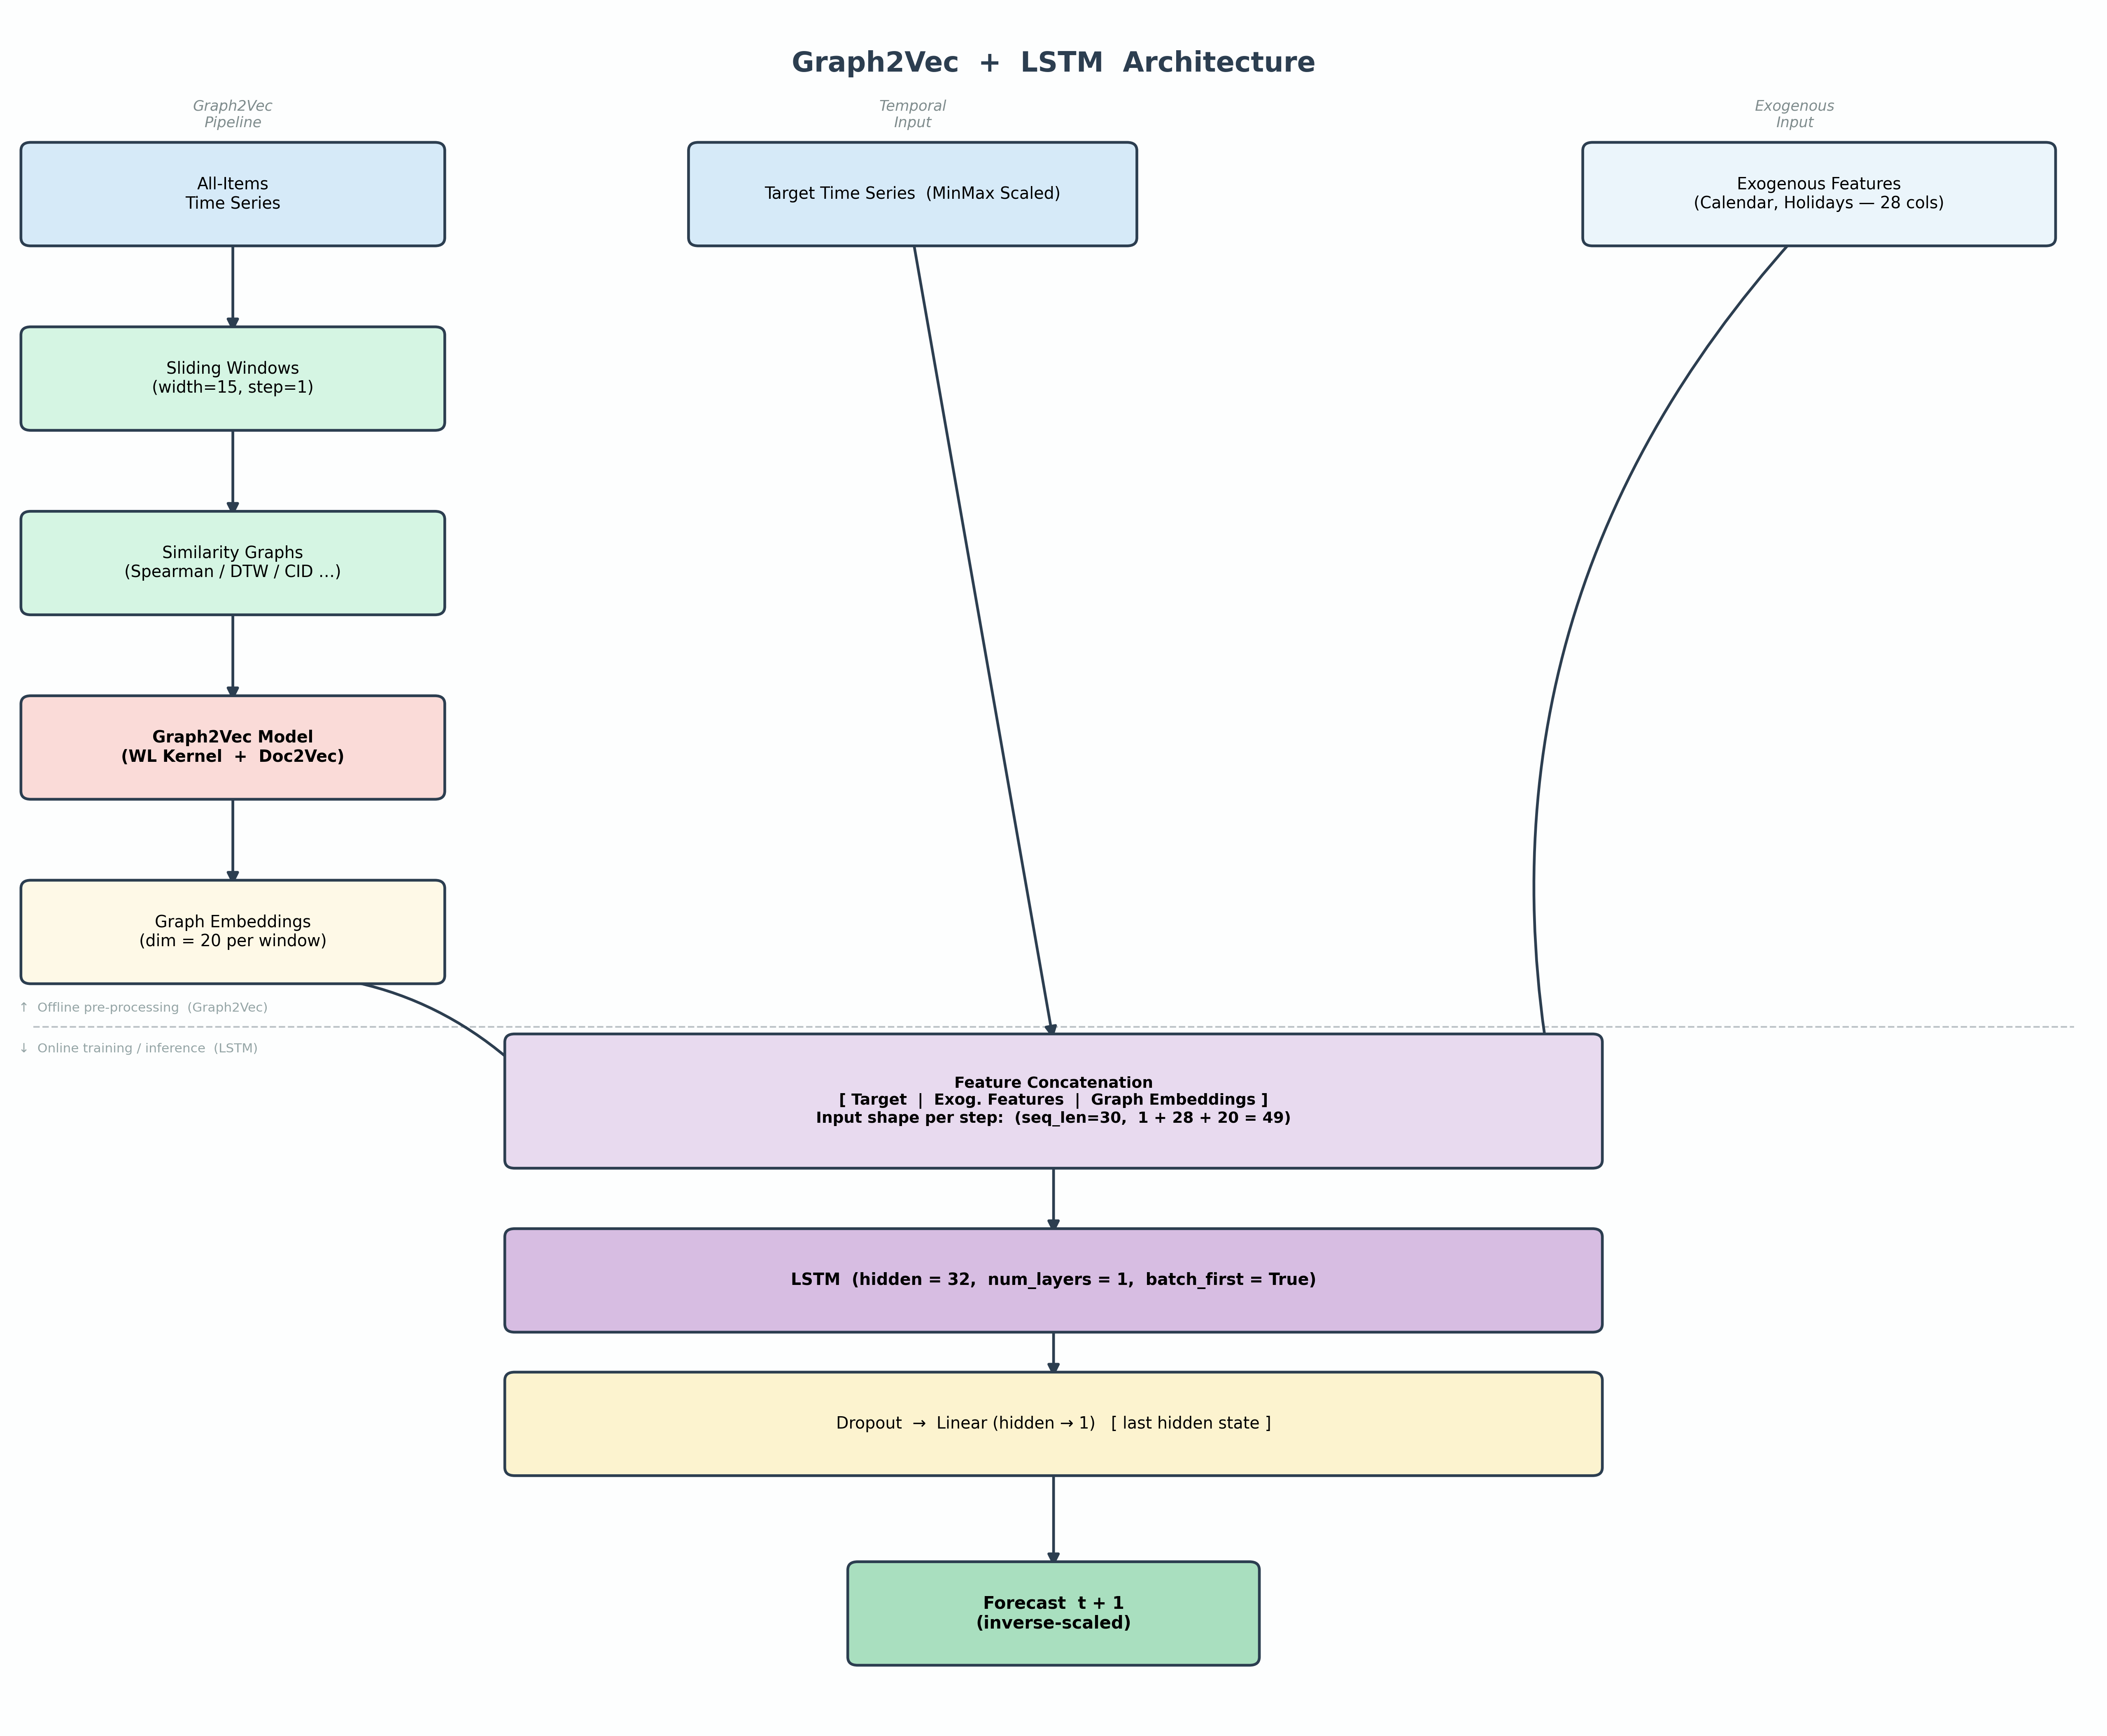
\includegraphics[width=\linewidth]{figures/Graph2VecLSTM.png}
        \caption{Graph2Vec-LSTM architecture.}
        \label{fig:graph2vec-lstm}
    \end{subfigure}
    \hfill
    \begin{subfigure}[t]{0.48\linewidth}
        \centering
        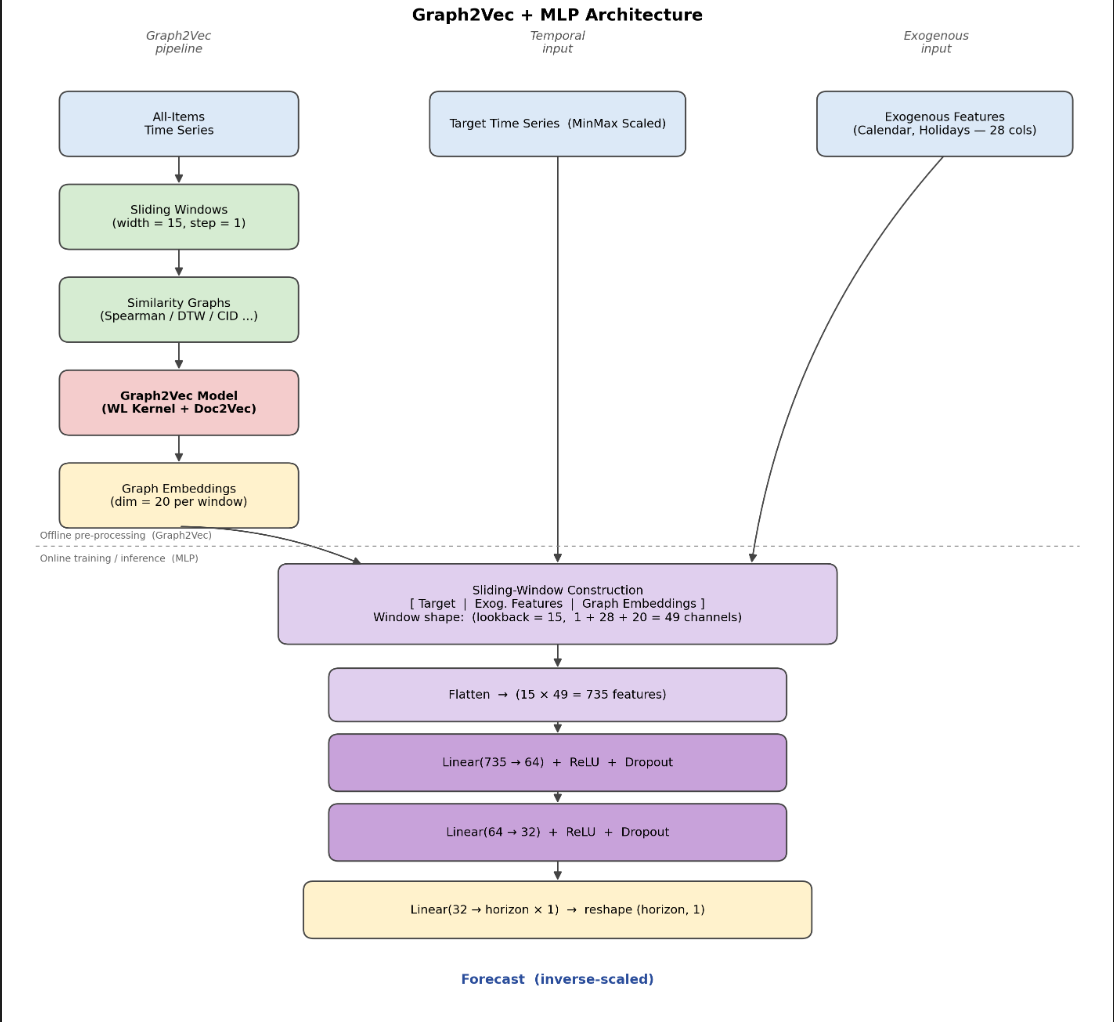
\includegraphics[width=\linewidth]{figures/Graph2Vec_MLP.png}
        \caption{Graph2Vec-MLP architecture.}
        \label{fig:graph2vec-mlp}
    \end{subfigure}

    \caption{Comparison of the Graph2Vec-based forecasting architectures.}
    \label{fig:graph2vec-comparison}
\end{figure}


To isolate the contribution of the relational signal, a \emph{no-embedding} baseline is run alongside every embedding configuration, using exactly the same target and exogenous features but with the embedding channel removed, providing an input size of \(1+28=29\). For each item--store--seed triplet, the grid search jointly varied the similarity metric and edge threshold while keeping the window size, step size, and LSTM hyperparameters fixed.


\section{GNN-Based End-to-End Strategies}

GNN-based end-to-end strategies have been designed to incorporate relational information directly into the forecasting process. Instead of relying only on the historical demand of an individual product, these approaches represent each target product as part of a dynamic graph, where the neighboring nodes correspond to products with similar temporal behaviors. This allows the model to learn not only from the target product's own demand pattern but also from the demand evolution of related products.

The main motivation for this strategy is that product demand is often influenced by shared patterns across items, such as common seasonality, similar sales cycles, category-level behavior, or correlated responses to calendar effects. A purely sequential model, such as an LSTM, or a purely feature-based model, such as an MLP, may fail to explicitly capture these relationships. Using a graph neural network, the forecasting model can aggregate information from similar products and learn a representation that reflects both temporal and structural dependencies.

In this study, a GNN-based strategy was implemented as an end-to-end hybrid architecture. The graph component learns a representation of the target product from its ego-graph, whereas the forecasting component combines this graph representation with the target product's recent time-series window and exogenous calendar features. The complete model is trained directly with the forecasting objective, meaning that the graph representation is optimized to improve the prediction accuracy rather than being computed as a separate, fixed embedding.

During inference, the model follows a recursive-forecasting procedure. At each step, the most recent demand window is used to rebuild the graph, the model predicts the next value, and the prediction is appended to the input window for the next step. This process allows the graph structure and temporal input to evolve throughout the multi-step forecast horizon, making the approach suitable for dynamic demand-forecasting scenarios.

\subsection{GCN}

A Graph Convolutional Network (GCN) is used as the graph-learning component of the proposed end-to-end hybrid strategy. For each target product, an ego graph is constructed by connecting the target node to other products whose historical demand patterns are considered similar according to a selected similarity or distance metric. The target product is always represented as the central node, whereas the neighboring nodes provide additional contextual information about the related demand behavior.

Each node in the graph contains time-series features extracted from a sliding window. Edges between nodes are weighted according to the similarity score between products. Therefore, stronger relationships have a greater influence during the graph convolution process.

The GCN branch applies graph convolutional layers to propagate and aggregate information across the ego-graph. Through this process, the representation of the target node is updated using information from its neighbouring products. The resulting target-node embedding captures relational demand patterns that are not available when modelling the target series in isolation.

This graph-based embedding is then combined with a separate temporal representation of the target product. The temporal branch receives the recent lookback window together with exogenous variables, such as calendar-related features, and projects them into a latent representation. The GCN embedding and the temporal projection are normalised, concatenated, and passed through an MLP prediction head to produce the next-step forecast.

The role of the GCN is therefore to enrich the forecasting model with information from structurally related products. By learning from both the target product and its dynamically selected neighbours, the model can better capture shared demand patterns and improve robustness in cases where the individual time series is noisy, sparse, or affected by irregular fluctuations.

\subsection{Node Feature Computation}

A central design choice in the GCN branch concerns how each node in the
ego-graph is described. In every configuration the features are extracted from
the same sliding window of raw demand used to construct the graph: given a
window of width $W$, each node $i$ is associated with its demand
sub-sequence $\mathbf{x}_i \in \mathbb{R}^{W}$ over that window.

\subsubsection{catch22 and catch24}

The node-feature representation used throughout this work is based on
\textit{catch22} (CAnonical Time-series CHaracteristics)
\cite{Lubba2019}, a curated set of 22
features selected for their discriminative power and low mutual redundancy
across diverse time-series classification tasks.  The features summarise
higher-order temporal properties of the window---autocorrelation structure,
distribution shape, entropy, linear and non-linear predictability, and
measures of stationarity---yielding a compact, fixed-length descriptor whose
dimensionality does not grow with the window length $W$.

A key property of \textit{catch22} is that it internally z-normalises each
series before computing its features, so that all information about the
absolute scale and level of the demand is, by design, removed.  While this
makes the representation invariant to demand magnitude and therefore more
transferable across products with very different sales volumes, it also means
that a node's feature vector carries no signal about how large or small the
recent demand actually was---information that is directly relevant to
forecasting.

To address this, the \texttt{pycatch22} library exposes a \texttt{catch24}
flag that appends two additional statistics---\texttt{DN\_Mean} (the arithmetic
mean of the raw window) and \texttt{DN\_Spread\_Std} (its standard
deviation)---to the 22 shape and dynamics features, producing a 24-dimensional
descriptor.  These two statistics are computed on the original, non-normalised
series and therefore reintroduce the scale and spread of demand that the
\textit{catch22} normalisation had discarded.

\subsubsection{Adding Explicit Scale Anchors: min, max, and last}

Although \texttt{DN\_Mean} and \texttt{DN\_Spread\_Std} partially recover
scale information, they characterise the distribution of the window in
aggregate and do not directly expose the extremes or the most recent level of
demand.  In practice, the minimum and maximum of the window bound the range of
observed values and are directly interpretable by message-passing operations,
while the last observation in the window---the value immediately preceding the
current forecast step---provides the most recent context and is often the
single strongest short-term predictor.

The final feature vector therefore concatenates the 24-dimensional catch24
block with three explicit scale anchors:
\[
\mathbf{f}_i = \bigl[\,\underbrace{c_{i,1},\ldots,c_{i,22}}_{\text{catch22}},\;
\underbrace{\mu_i,\;\sigma_i}_{\text{DN\_Mean/Std}},\;
\underbrace{\min_i,\;\max_i,\;x_i^{(W-1)}}_{\text{scale anchors}}\,\bigr]
\;\in\;\mathbb{R}^{27},
\]
where $\mu_i$ and $\sigma_i$ are the mean and standard deviation of the raw
window (the catch24 additions), $\min_i$ and $\max_i$ its extrema, and
$x_i^{(W-1)}$ the last observed value.  This 27-dimensional representation
combines the rich temporal shape information of \textit{catch22} with
sufficient scale context to allow the graph convolution to propagate both the
dynamics and the demand level of each neighbour to the target node.

{\small\sloppy
\setlength{\tabcolsep}{4pt}% tighter columns
\renewcommand{\arraystretch}{1.05}% a touch more leading
\begin{longtable}{@{}c
  >{\ttfamily\raggedright\arraybackslash}p{0.30\linewidth}
  >{\raggedright\arraybackslash}p{0.18\linewidth}
  >{\raggedright\arraybackslash}p{0.40\linewidth}
  c@{}}
\caption{Node-feature vector for the \texttt{catch24\_minmaxlast} mode.
         Features 0--21 are the 22 \textit{catch22} features returned by
         \texttt{pycatch22} in their library order; features 22--23 are the
         two scale statistics appended by the \texttt{catch24=True} flag;
         features 24--26 are the three explicit scale anchors added by this
         work.  The \textit{Zeroed} column indicates whether a feature was
         observed as zero for the target node in the illustrative window:
         $\circ$~=~structural zero (no outliers detected),
         $\bullet$~=~NaN replaced by zero (numerical failure of the
         log-linear fit on a short window).}
\label{tab:node_features} \\
\toprule
\# & Feature code & Category & Description & Zeroed \\
\midrule
\endfirsthead
\toprule
\# & Feature code & Category & Description & Zeroed \\
\midrule
\endhead
\midrule
\multicolumn{5}{r}{\footnotesize Continued on next page} \\
\endfoot
\bottomrule
\endlastfoot

\multicolumn{5}{l}{\textit{catch22 features (indices 0--21, scale-invariant)}} \\[2pt]
 0 & DN\_\allowbreak HistogramMode\_\allowbreak 5                          & Distribution shape         & Mode of 5-bin histogram of z-normalised series               & ---           \\
 1 & DN\_\allowbreak HistogramMode\_\allowbreak 10                         & Distribution shape         & Mode of 10-bin histogram of z-normalised series              & ---           \\
 2 & CO\_\allowbreak f1ecac                                    & Autocorrelation            & First $1/e$ crossing of the ACF                              & ---           \\
 3 & CO\_\allowbreak FirstMin\_\allowbreak ac                              & Autocorrelation            & First minimum of the ACF (lag index)                         & ---           \\
 4 & CO\_\allowbreak HistogramAMI\_\allowbreak even\_\allowbreak 2\_\allowbreak 5                  & Nonlinear autocorrelation  & Auto-mutual information, lag 2, 5 bins                       & ---           \\
 5 & CO\_\allowbreak trev\_\allowbreak 1\_\allowbreak num                              & Nonlinear autocorrelation  & Time-reversibility statistic                                 & ---           \\
 6 & MD\_\allowbreak hrv\_\allowbreak classic\_\allowbreak pnn40                       & Incremental differences    & Proportion of successive differences $>{0.4}\sigma$          & ---           \\
 7 & SB\_\allowbreak BinaryStats\_\allowbreak mean\_\allowbreak longstretch1           & Symbolic                   & Length of longest above-mean stretch                         & ---           \\
 8 & SB\_\allowbreak TransitionMatrix\_\allowbreak 3ac\_\allowbreak sumdiagcov         & Symbolic                   & Column variance of 3-symbol transition matrix                & ---           \\
 9 & PD\_\allowbreak PeriodicityWang\_\allowbreak th0\_\allowbreak 01                  & Periodicity                & Wang's periodicity metric (dominant lag)                     & ---           \\
10 & CO\_\allowbreak Embed2\_\allowbreak Dist\_\allowbreak tau\_\allowbreak d\_\allowbreak expfit\_\allowbreak meandiff    & Nonlinear                  & Mean diff.\ of exponential fit to 2-D embedding distances    & ---           \\
11 & IN\_\allowbreak AutoMutualInfoStats\_\allowbreak 40\_\allowbreak gaussian\_\allowbreak fmmi   & Autocorrelation structure  & First minimum lag of the AMI function                        & ---           \\
12 & FC\_\allowbreak LocalSimple\_\allowbreak mean1\_\allowbreak tauresrat              & Forecasting                & Change in ACF timescale after first-differencing             & ---           \\
13 & DN\_\allowbreak OutlierInclude\_\allowbreak p\_\allowbreak 001\_\allowbreak mdrmd             & Extreme event timing       & Mean deviation from median (positive outliers only)          & $\circ$       \\
14 & DN\_\allowbreak OutlierInclude\_\allowbreak n\_\allowbreak 001\_\allowbreak mdrmd             & Extreme event timing       & Mean deviation from median (negative outliers only)          & ---           \\
15 & SP\_\allowbreak Summaries\_\allowbreak welch\_\allowbreak rect\_\allowbreak area\_\allowbreak 5\_\allowbreak 1        & Spectral                   & Power in the lowest 20\% of frequencies (Welch)              & ---           \\
16 & SB\_\allowbreak BinaryStats\_\allowbreak diff\_\allowbreak longstretch0           & Symbolic                   & Length of longest monotonically decreasing stretch           & ---           \\
17 & SB\_\allowbreak MotifThree\_\allowbreak quantile\_\allowbreak hh                  & Symbolic                   & Entropy of successive pairs in quantile-symbolised series    & ---           \\
18 & SC\_\allowbreak FluctAnal\_\allowbreak 2\_\allowbreak rsrangefit\_\allowbreak 50\_\allowbreak 1\_\allowbreak logi\_\allowbreak prop\_\allowbreak r1 & Self-affine scaling        & Rescaled-range fluctuation analysis (low-scale regime)       & $\bullet$     \\
19 & SC\_\allowbreak FluctAnal\_\allowbreak 2\_\allowbreak dfa\_\allowbreak 50\_\allowbreak 1\_\allowbreak 2\_\allowbreak logi\_\allowbreak prop\_\allowbreak r1    & Self-affine scaling        & Detrended fluctuation analysis (low-scale regime)            & $\bullet$     \\
20 & SP\_\allowbreak Summaries\_\allowbreak welch\_\allowbreak rect\_\allowbreak centroid          & Spectral                   & Centroid frequency of the power spectrum                     & ---           \\
21 & FC\_\allowbreak LocalSimple\_\allowbreak mean3\_\allowbreak stderr                & Forecasting                & Residual std.\ of 3-point rolling-mean forecast              & ---           \\[4pt]

\multicolumn{5}{l}{\textit{catch24 additions (indices 22--23, raw-scale)}} \\[2pt]
22 & DN\_\allowbreak Mean                                      & Scale recovery             & Arithmetic mean of the raw window ($\mu_i$)                  & ---           \\
23 & DN\_\allowbreak Spread\_\allowbreak Std                               & Scale recovery             & Standard deviation of the raw window ($\sigma_i$)            & ---           \\[4pt]

\multicolumn{5}{l}{\textit{Explicit scale anchors (indices 24--26, raw-scale)}} \\[2pt]
24 & min                                           & Scale anchor               & Minimum value in the raw window ($\min_i$)                   & ---           \\
25 & max                                           & Scale anchor               & Maximum value in the raw window ($\max_i$)                   & ---           \\
26 & last                                          & Scale anchor               & Last (most recent) value in the raw window ($x_i^{(W-1)}$)  & ---           \\

\end{longtable}
}

\subsubsection{Robustness and Dynamic Recomputation}

Several \textit{catch22} features are mathematically ill-defined on
near-constant or very short windows and return \texttt{NaN}, while strictly
constant series can additionally fail in the underlying extraction backend.
To prevent a single degenerate node from corrupting the entire graph during
message passing, any non-finite feature is replaced by zero and a node whose
extraction fails entirely falls back to an all-zero feature vector.

In the illustrative window detailed in Table \ref{tab:node_features}, this fallback mechanism is explicitly demonstrated by the zeroing of three specific features. The extreme event timing metric (\texttt{DN \_OutlierInclude \_p \_001 \_mdrmd}, index 13) resolves to a structural zero (\(\circ\)) simply because no positive outliers exist within that specific time frame. By contrast, the two self-affine scaling metrics---rescaled-range and detrended fluctuation analyses (indices 18 and 19)---initially yield \texttt{NaN} values that the system actively replaces with zero (\(\bullet\)). These numerical failures occur because the short length of the rolling window provides insufficient data points to compute the robust log-linear fits required across multiple scales, practically necessitating the \texttt{NaN}-to-zero safeguard during localized extraction.
Regardless of the window, the node features are recomputed dynamically as the
graph evolves.  During the recursive multi-step forecast the target node's
feature row is refreshed at each step from the rolling demand window, where
the most recent observation is replaced by the model's own prediction rather
than the ground-truth value.  The same 27-dimensional transformation is
therefore applied consistently at both training and inference time, ensuring
that no test-period information leaks into the node features while the graph
structure and node descriptors are updated throughout the forecast horizon.

\subsubsection{Link to LSTM Training}

The GCN and the LSTM are not trained as separate stages. Instead, they form a
single end-to-end network in which the graph encoder, the recurrent encoder,
and the prediction head are optimised jointly under one forecasting loss. The
GCN does not produce a fixed, precomputed embedding; rather, its parameters are
updated by the same gradient signal that trains the LSTM, so that the learned
graph representation is shaped specifically to improve the forecast.

\paragraph{Per-step coupling of the two branches.}
The two branches are coupled at every step of the lookback window. For a
lookback length $L$, each training sample carries $L$ ego-graphs, one per
lookback day, aligned so that the graph used at step $i$ is built strictly from
the days preceding it (preventing label leakage). During a forward pass, a
batch of $B$ samples is flattened into $B \times L$ ego-graphs and encoded by
the GCN in a single sparse operation. Two graph-convolutional layers propagate
information across each ego-graph, and the embedding of the target node (row $0$
of every subgraph, recovered through the batch pointer indices) is extracted
and passed through a layer normalisation, yielding a per-step graph vector
$\mathbf{z} \in \mathbb{R}^{d_g}$. These vectors are reshaped back to
$(B, L, d_g)$ in the same row-major order produced by the collation step, so
that each lookback day is paired with the graph embedding computed for that day.

\paragraph{Fusion before the recurrence.}
The graph embedding is fused with the temporal input \emph{before} the LSTM
processes the sequence. At each step the model concatenates the target value,
the exogenous calendar features, and the corresponding graph embedding into a
single augmented vector,
\[
\mathbf{x}_t = \big[\, y_t \;\Vert\; \mathbf{e}_t \;\Vert\; \mathbf{z}_t \,\big]
\in \mathbb{R}^{1 + n_\text{exog} + d_g},
\]
and the resulting sequence $(\mathbf{x}_1, \dots, \mathbf{x}_L)$ is fed to the
LSTM. Because the relational signal enters the recurrence as additional
input features at every step, the LSTM can integrate structural information
from related products together with the target's own temporal dynamics, rather
than treating the graph embedding as a static side input. The hidden state of
the final step is passed through dropout and a linear head to produce the
next-step prediction.

\paragraph{Backpropagation through both branches.}
Training minimises a single forecasting loss (mean squared error) between the
final-step prediction and the ground-truth target, with the same mean squared
error used for validation and early stopping. The optimiser is bound to all model
parameters at once, so a single call to backpropagation propagates gradients
from the prediction head, back through the LSTM, through the concatenation that
fused the two branches, and into the GCN convolutional layers and the layer
normalisation. The concatenation is the point at which the error signal splits:
part of it flows along the temporal path into the LSTM weights, and part flows
along the structural path into the GCN weights and, through the edge-weighted
message passing, shapes how neighbour information is aggregated. The graph
representation is therefore learned discriminatively for the forecasting
objective, not as an unsupervised or pretext embedding.

\paragraph{Training stabilisation and diagnostics.}
Several mechanisms keep the joint optimisation stable. Layer normalisation on
$\mathbf{z}$ prevents the magnitude of the graph embedding from dominating or
collapsing relative to the temporal features at the fusion point. Global
gradient-norm clipping bounds the combined gradient before each optimiser
update, and dropout is applied in the GCN, the LSTM, and the head to limit
overfitting. To monitor the relative contribution of the two branches during
training, the loop separately accumulates the gradient norms of the
graph-related parameters (the convolutional layers and $\mathbf{z}$
normalisation) and of the LSTM parameters, and logs their ratio together with
the mean norm and variance of the captured $\mathbf{z}$ embeddings. These
diagnostics make it possible to verify that the graph branch is actually
receiving and using a meaningful share of the learning signal rather than being
ignored. An ablation switch is also provided that zeroes the graph embedding
before fusion, reducing the architecture to a purely temporal LSTM and allowing
the contribution of the GCN branch to be measured directly.

\paragraph{Recursive inference.}
Since the model forecasts a single step ahead, multi-step predictions are
generated by recursive roll-out. At inference the model maintains a rolling
deque of $L$ ego-graphs alongside the $L$-row lookback window, mirroring the
per-step layout used during training. At each step it is queried on the current
(\,$L$-graph deque, $L$-row temporal window\,) pair to predict the next value
$\hat{y}$; the lookback window is then advanced by dropping the oldest target
value and appending $\hat{y}$, while the exogenous row is moved to the calendar
features of the day being predicted, and the graph deque is advanced by dropping
the oldest graph and appending the ego-graph aligned to that same day. Both the
temporal input and the underlying graph structure therefore evolve jointly
across the horizon rather than being held fixed. To keep the forecast strictly
causal and free of label leakage, the target node's feature row of each newly
appended graph is recomputed from a rolling window of the model's \emph{own}
predictions, where $\hat{y}$ is inverse-scaled, re-scaled with the target
product's scaler, and used to regenerate the node features through the same
transformation chosen at training time ; the same own-prediction history
is used to refresh any leakage-prone exogenous features such as demand lags and
rolling means. The predictions are finally inverse-transformed back to the
original demand scale, so the GCN+LSTM is rolled out autoregressively while
preserving identical, causal train- and test-time semantics over the entire
forecast horizon.

\begin{figure}[!htbp]
    \centering
    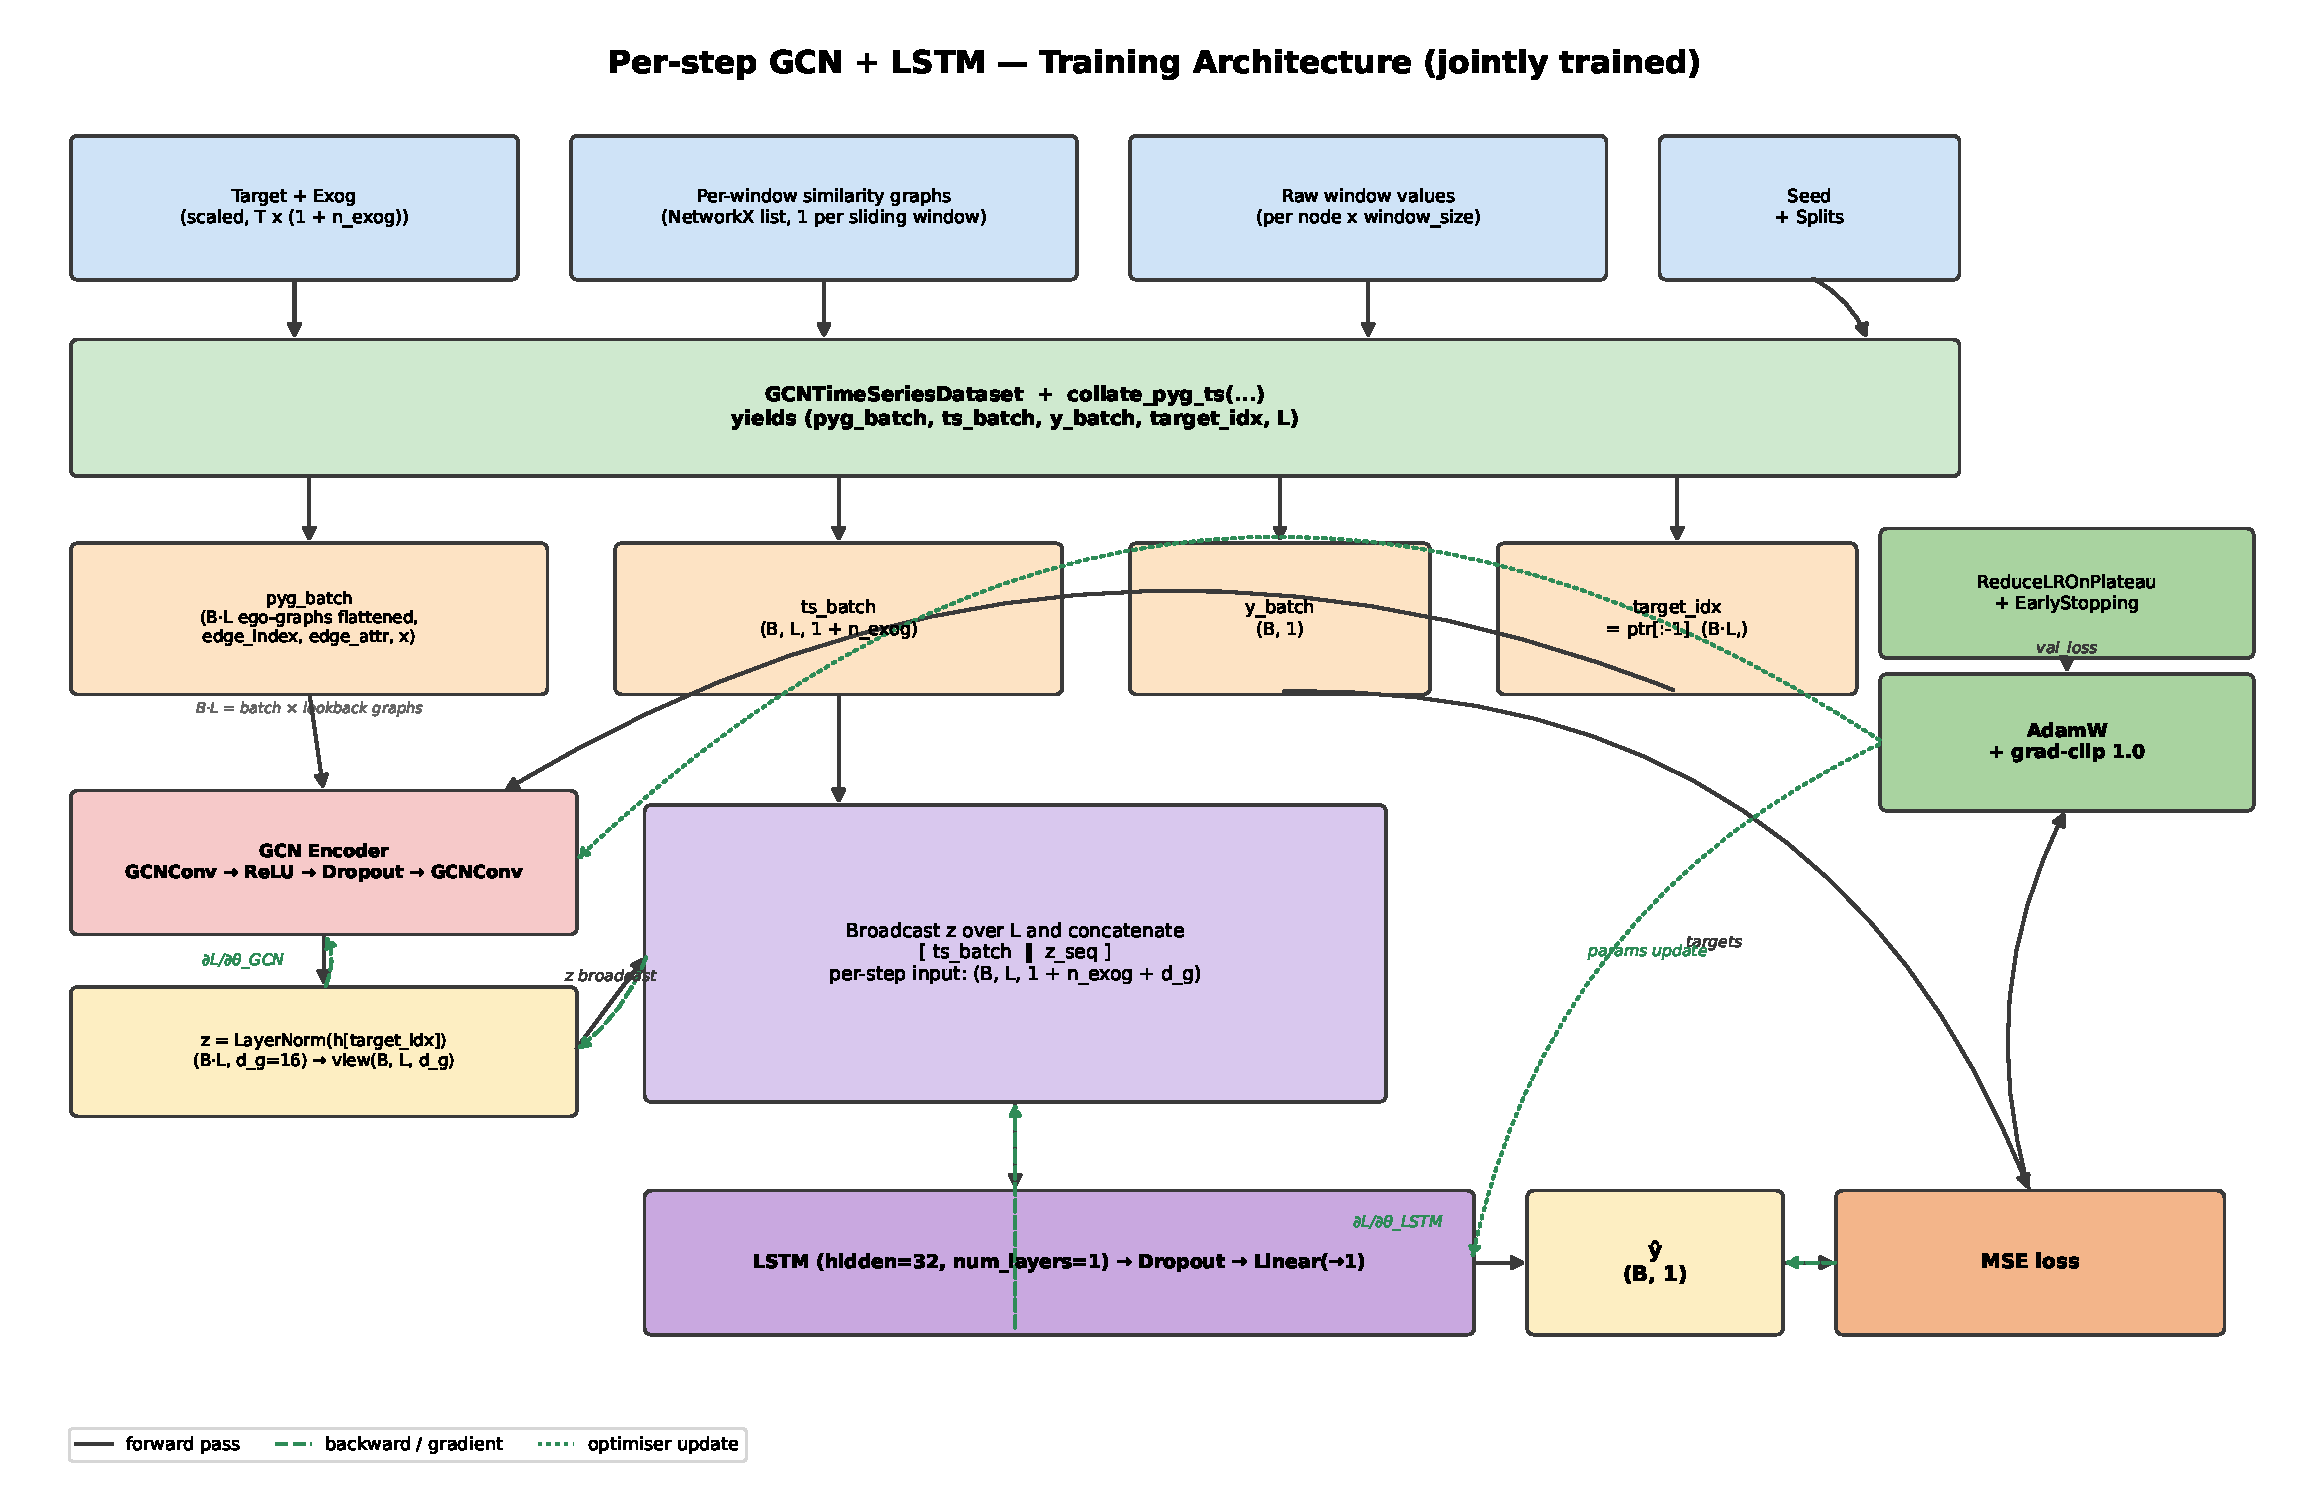
\includegraphics[width=0.8\linewidth]{figures/gcn_lstm_training_architecture.pdf}
    \caption{End-to-end training architecture of the per-step GCN + LSTM forecaster. The model is trained jointly: gradients from the forecasting loss flow back through both the temporal (LSTM) and the graph (GCN) branches in a single optimisation. Inputs (top row): the scaled target series augmented with exogenous calendar/holiday features ($T \times (1 + n_{\text{exog}})$); a list of per-window similarity/distance graphs (one NetworkX graph per sliding window, here built from Spearman dynamic similarity over the training period); the raw per-node window values used to compute node features (catch24 + scale/level extras); and the random seed plus train/validation/test splits. Batching: GCNTimeSeriesDataset together with the per-step collator collate\_pyg\_ts materialises each minibatch as four tensors --- pyg\_batch, a flattened $B \cdot L$ ego-graphs (one ego-graph per lookback day, $B$ samples $\times L$ lookback steps, with edge\_index, edge\_attr, node features $x$); ts\_batch $(B, L, 1 + n_{\text{exog}})$; the regression targets $y_{\text{batch}}$ $(B, 1)$; and target\_idx $= \text{ptr}[:-1]$, the $(B \cdot L,)$ indices selecting each subgraph's target (ego) node within the batched node matrix. GCN branch: a two-layer encoder (GCNConv $\rightarrow$ ReLU $\rightarrow$ Dropout $\rightarrow$ GCNConv) embeds all $B \cdot L$ graphs in one sparse pass; the target-node rows are gathered via target\_idx and LayerNorm-normalised to give the per-step embeddings $z$ $(B \cdot L, d_g = 16)$, which are reshaped to $(B, L, d_g)$ in the same row-major order produced by the collator so that each lookback day is paired with its own graph embedding. Fusion: the reshaped per-step embeddings $z$ $(B, L, d_g)$ are concatenated with ts\_batch at each step, forming the per-step LSTM input of width $1 + n_{\text{exog}} + d_g$. Temporal head: a single-layer LSTM (hidden $= 32$) followed by Dropout and a Linear($\rightarrow 1$) layer maps the last hidden state to the one-step-ahead prediction $\hat{y}$ $(B, 1)$. Optimisation: the prediction is compared to $y_{\text{batch}}$ under an MSE loss; parameters of both branches are updated with AdamW (gradient-norm clipping at $1.0$), the learning rate annealed by ReduceLROnPlateau on the validation loss, with early stopping on the same signal. Line styles distinguish the forward pass (solid), backward/gradient flow (dashed; $\partial L/\partial \theta_{\text{LSTM}}$ and $\partial L/\partial \theta_{\text{GCN}}$ reach both branches, confirming end-to-end joint training) and the optimiser parameter update (dotted).}
    \label{fig:gcn_lstm_training_architecture}
\end{figure}

\subsubsection{Link to MLP Training}
\label{sec:gcn_mlp_link}

As in the recurrent variant, the GCN and the MLP are not trained as separate
stages. They form a single end-to-end network, \texttt{SimpleGCNMLPForecaster},
in which the graph encoder, a shared time-distributed MLP, and the prediction
head are optimised jointly under one forecasting loss. The GCN does not produce
a fixed, precomputed embedding; its parameters are updated by the same gradient
that trains the MLP, so the learned graph representation is shaped specifically
to improve the forecast.

\paragraph{Per-step coupling of the two branches.}
The two branches are coupled at every step of the lookback window. For a
lookback length $L$, each training sample carries $L$ ego-graphs, one per
lookback day, aligned so that the graph used at step $i$ is built strictly from
the days preceding it (preventing label leakage). During a forward pass, a
batch of $B$ samples is flattened into $B \times L$ ego-graphs and encoded by
the GCN in a single sparse operation. Two edge-weighted graph-convolutional
layers (with self-loops, ReLU and dropout in between) propagate information
across each ego-graph, and the embedding of the target node (row $0$ of every
subgraph, recovered through the batch pointer indices) is extracted and passed
through a layer normalisation, yielding a per-step graph vector
$\mathbf{z}_t \in \mathbb{R}^{d_g}$. These vectors are reshaped back to
$(B, L, d_g)$ in the same row-major order produced by the collation step, so
that each lookback day is paired with the graph embedding computed for that day.

\paragraph{Fusion before the head.}
The graph embedding is fused with the temporal input \emph{per step}, before
the MLP processes the sequence. At each step the model concatenates the target
value, the exogenous calendar features, and the corresponding graph embedding
into a single augmented vector,
\[
\mathbf{x}_t = \big[\, y_t \;\Vert\; \mathbf{e}_t \;\Vert\; \mathbf{z}_t \,\big]
\in \mathbb{R}^{1 + n_\text{exog} + d_g},
\]
giving an augmented sequence $(\mathbf{x}_1, \dots, \mathbf{x}_L)$. Crucially,
this sequence is \emph{not flattened} into one long vector, and there is no
separate linear projection of the lookback: the relational signal enters as
additional per-step features, exactly as in the recurrent variant, the only
difference being how the augmented sequence is subsequently consumed.

\paragraph{Time-distributed MLP head.}
Instead of a recurrence, a single shared MLP (a stack of
\texttt{Linear $\to$ ReLU $\to$ Dropout} blocks) is applied independently and
with identical weights to each of the $L$ augmented steps, mapping
$\mathbf{x}_t \mapsto \mathbf{h}_t$. This time-distributed design keeps the
head invariant to the lookback length and lets the network learn one per-step
transformation that is reused across the window, rather than learning a
position-specific mapping over a flattened input. The $L$ step
representations are then pooled by concatenating the most recent step with the
mean over all steps,
\[
\mathbf{g} = \big[\, \mathbf{h}_L \;\Vert\; \tfrac{1}{L}\textstyle\sum_{t=1}^{L}\mathbf{h}_t \,\big],
\]
combining the latest local context with a global summary of the window, and a
final linear layer maps $\mathbf{g}$ to the forecast horizon $H$.

\paragraph{Backpropagation through both branches.}
Training minimises a single forecasting loss (e.g.\ mean squared error) between
the final-step prediction and the ground-truth target, with a separate metric
used for validation and early stopping. The optimiser is bound to all model
parameters at once, so a single backward pass propagates gradients from the
linear head, back through the pooled representation and the shared per-step MLP,
through the concatenation that fused the two branches, and into the GCN
convolutional layers and the layer normalisation. The concatenation is the
point at which the error signal splits: part flows along the temporal path into
the MLP weights, and part flows along the structural path into the GCN weights
and, through the edge-weighted message passing, shapes how neighbour
information is aggregated. The graph representation is therefore learned
discriminatively for the forecasting objective, not as an unsupervised or
pretext embedding.

\paragraph{Training stabilisation and diagnostics.}
The same stabilisation mechanisms as the recurrent variant apply. Layer
normalisation on $\mathbf{z}$ prevents the magnitude of the graph embedding
from dominating or collapsing relative to the temporal features at the fusion
point. Global gradient-norm clipping bounds the combined gradient before each
optimiser update, and dropout is applied in both the GCN and the MLP. To
monitor the relative contribution of the two branches, the training loop
separately accumulates the gradient norms of the graph-related parameters
(the convolutional layers and the $\mathbf{z}$ normalisation) and of the MLP
parameters, and logs their ratio together with the mean norm and variance of
the captured $\mathbf{z}$ embeddings, verifying that the graph branch receives
a meaningful share of the learning signal. An ablation switch is also provided
that zeroes the graph embedding before fusion, reducing the architecture to a
purely temporal time-distributed MLP and allowing the GCN contribution to be
measured directly.

\paragraph{Recursive inference.}
At test time the fused model is rolled out one step at a time. A deque of $L$
ego-graphs is maintained alongside the lookback window: at each step the model
predicts the next value, the prediction is appended to the lookback (and to the
unscaled history used for any leakage-safe lag and rolling-mean features), and
the graph deque is advanced by dropping the oldest graph and appending the
graph aligned to the day just predicted. To avoid label leakage, the target
node's feature row in each newly appended graph is overwritten with features
derived from the model's own rolling predictions rather than ground-truth test
values. The same forward signature
$\texttt{model}(G_t, \mathbf{s}_t) \rightarrow (B, H, 1)$ is used during
training and inference, so train- and test-time semantics are identical and the
graph information is exploited consistently throughout the forecast horizon.

\begin{figure}[!htbp]
    \centering
    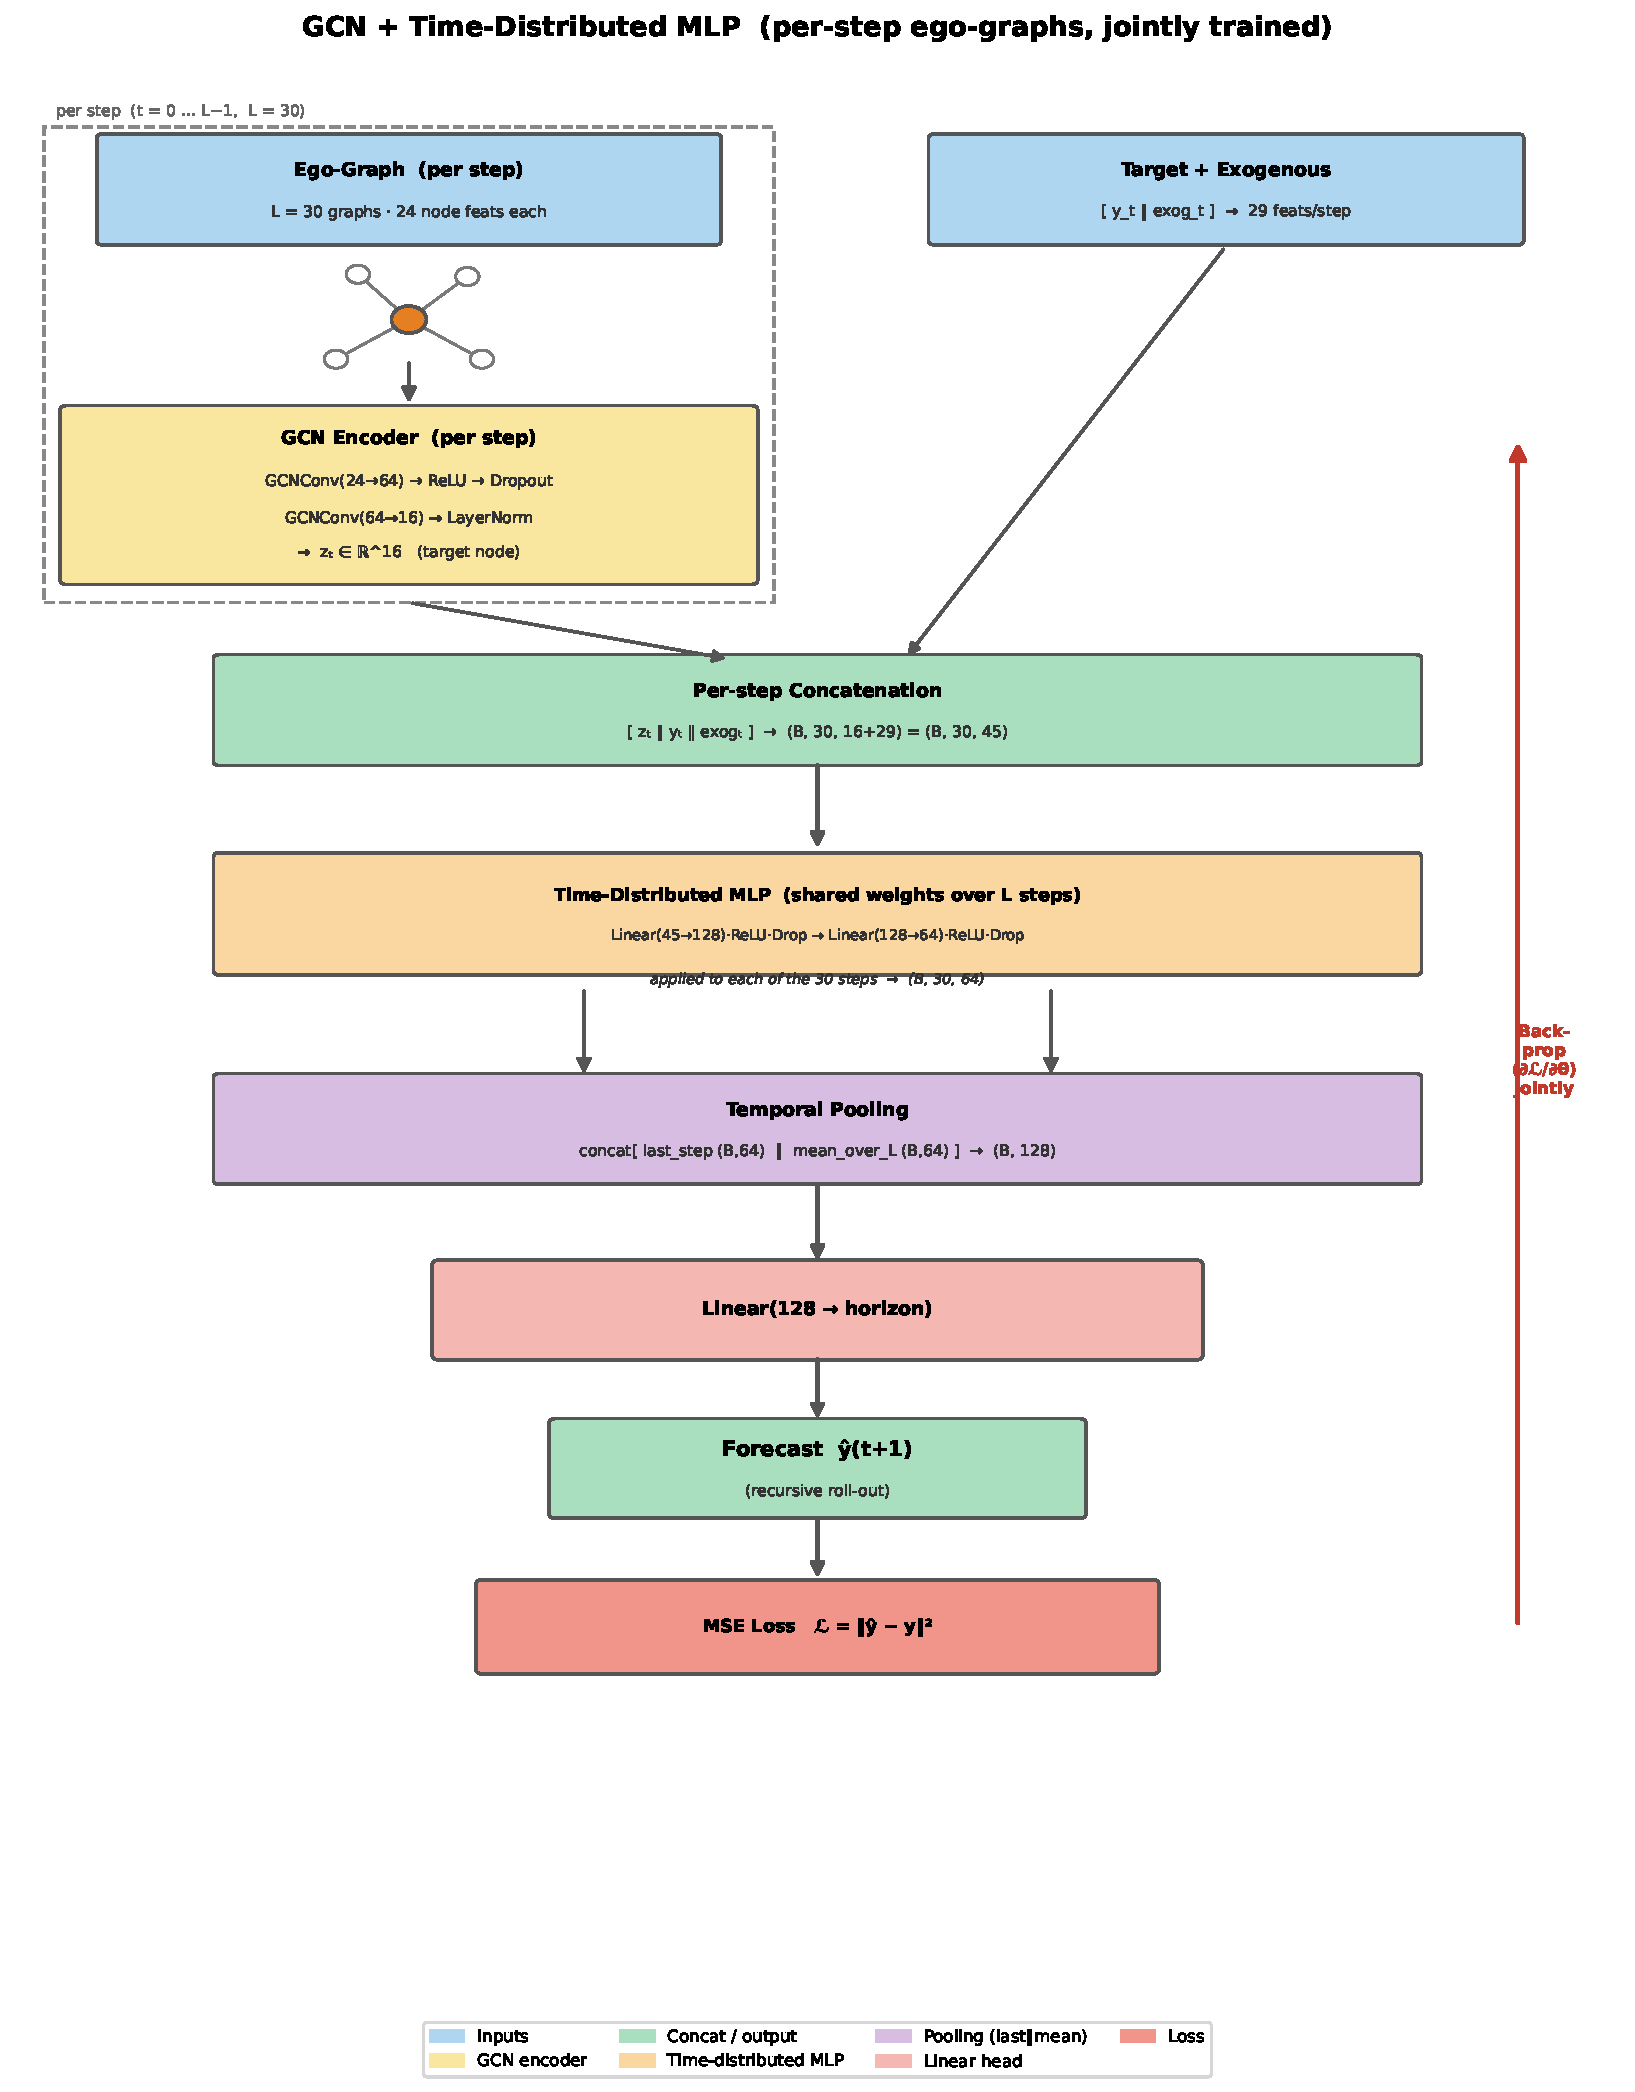
\includegraphics[width=0.5\linewidth]{figures/gcn_tdmlp_architecture.pdf}
    \caption{Architecture of the per-step GCN + time-distributed MLP forecaster (GCN--TDMLP), trained end-to-end. For each lookback day $t$ in a window of length $L=30$, an ego-graph is built around the target item and its neighbours; each node uses a 24-dimensional \texttt{catch24} feature vector. A weight-shared two-layer GCN encoder (GCNConv $24\!\to\!64$ $\to$ ReLU $\to$ Dropout $\to$ GCNConv $64\!\to\!16$ $\to$ LayerNorm) produces a target-node embedding $\mathbf{z}_t\in\mathbb{R}^{16}$. Per step, the fused input is $[\mathbf{z}_t\,\Vert\, y_t\,\Vert\, \mathbf{x}^{\text{exog}}_t]$, giving a sequence tensor of shape $(B,L,16+1+n_{\text{exog}})$, where $B$ is the minibatch size, $y_t$ is the (scaled) target value, and $\mathbf{x}^{\text{exog}}_t\in\mathbb{R}^{n_{\text{exog}}}$ are exogenous features. A time-distributed MLP (Linear $\to$ ReLU $\to$ Dropout $\to$ Linear $\to$ ReLU $\to$ Dropout) maps each step to $(B,L,64)$, then temporal pooling forms $[\mathbf{h}_{\text{last}}\,\Vert\,\text{mean}(\mathbf{h}_{1:L})]\in\mathbb{R}^{128}$. A final Linear layer outputs a one-step prediction $\hat{y}_{t+1}$ (and, in general, $H$ steps for horizon $H$). The model is trained with MSE loss $\mathcal{L}$, with gradients backpropagated through both the MLP and GCN parameters.}
    \label{fig:gcn_tdmlp_architecture}
\end{figure}


\subsection{GAT}
To complement or serve as an alternative to the GCN layer, the architecture also implements a Graph Attention Network (GAT) branch. While the GCN aggregates neighbor information using a fixed, static weighting based solely on the pre-computed similarity metric, the GAT branch introduces a learned, dynamic aggregation strategy by explicitly utilizing multiple parallel attention heads.  In this branch, a custom edge-weighted GAT convolutional layer is utilized to process the ego-graph. Standard GAT implementations typically treat edge attributes merely as an additive bias within the attention calculation. However, to preserve the strong structural prior of the similarity network, the custom GAT multiplicatively gates its learned attention coefficients using the explicit edge weights. Specifically, the multi-head attention mechanism calculates softmax-normalised coefficients, which are then multiplied by the non-negative similarity edge weights and renormalised for each target node. This ensures that inherently low-similarity neighbors are heavily down-weighted regardless of the network's learned attention score, effectively marrying data-driven feature attention with the explicit graph topology. Furthermore, self-loops are strictly enforced with a maximum weight of 1.0, guaranteeing that the target product's own historical signal is maximally trusted and preserved during aggregation.  The GAT encoder is structured across two primary layers to process these relationships. In the first convolutional layer, the outputs from the multiple attention heads are concatenated to capture a wide, diverse array of relational features. A subsequent layer then aggregates these representations using a single attention head, averaging the outputs rather than concatenating them, to project the final target-node embedding down to the required latent dimension. Exactly like the GCN branch, this refined, attention-driven graph embedding is subsequently concatenated with the temporal and exogenous features before being passed through the recurrent layers and the final prediction head.  

\subsection{GCN vs GAT implementations}
While both the GCN and the GAT branches are designed to map the per-window ego-graphs into a target-node embedding of dimension $d_g$, their aggregation mechanisms and layer architectures differ fundamentally. The GCN branch employs a standard PyTorch Geometric GCNConv layer, which utilizes the pre-computed similarity scores as static, explicit edge weights during neighborhood aggregation. In contrast, the GAT branch utilizes a custom EdgeWeightedGATConv layer to marry data-driven attention with the explicit graph topology. Standard GAT implementations typically use edge attributes merely as an additive bias; however, this custom implementation multiplicatively gates the learned, softmax-normalized attention coefficients using the structural similarity weights, followed by per-node renormalization. Architecturally, the GAT branch deploys a multi-head mechanism in its first layer that concatenates the representations from parallel attention heads, requiring an ELU activation to preserve negative values. Its second layer then averages the multi-head outputs down to the target dimension. The GCN branch, being simpler, applies a single projection per layer followed by a standard ReLU activation. 

\begin{table}[htpb]
\centering
\caption{Architectural and implementation differences between the GCN and GAT branches.}
\label{tab:gcn_vs_gat}
\begin{tabular}{@{} l p{5cm} p{6.5cm} @{}}
\toprule
\textbf{Feature} & \textbf{GCN Branch} & \textbf{GAT Branch} \\
\midrule
\textbf{Base PyG Module} & \texttt{GCNConv} & Custom \texttt{EdgeWeightedGATConv} (extends \texttt{GATConv}) \\
\addlinespace
\textbf{Edge Weighting} & Uses similarity scores directly as static \texttt{edge\_weight} during aggregation. & Multiplicatively gates learned attention coefficients with similarity scores (\texttt{edge\_attr}), then renormalizes. \\
\addlinespace
\textbf{Layer 1 Structure} & Single projection. & Multi-head attention (default 4 heads); outputs are concatenated (\texttt{concat=True}). \\
\addlinespace
\textbf{Layer 2 Structure} & Single projection to dimension $d_g$. & Single head; outputs are averaged (\texttt{concat=False}) to dimension $d_g$. \\
\addlinespace
\textbf{Activation Function} & ReLU (\texttt{nn.ReLU}). & ELU (\texttt{nn.ELU}) to preserve negative values from concatenated attention heads. \\
\addlinespace
\textbf{Self-Loops} & Added automatically by \texttt{GCNConv}. & Explicitly forced to a maximum similarity value of 1.0 (\texttt{fill\_value=1.0}) so the target node strongly trusts its own signal. \\
\bottomrule
\end{tabular}
\end{table}